\documentclass[a4paper]{IEEEtran}
%\documentclass[a4paper, onecolumn]{IEEEtran}
\usepackage[T1]{fontenc}
\usepackage[utf8]{inputenc}
\usepackage[english]{babel}

\usepackage{authblk}
\usepackage{hyperref}
\usepackage{graphicx}
\usepackage{listings}
%\usepackage{amsmath}
\usepackage[cmex10]{amsmath}
\usepackage{amssymb}
%\usepackage{fullpage}
\usepackage{float}
\usepackage{url} \urlstyle{sf}

\usepackage{dashrule}

\usepackage{color}
\usepackage{subcaption}
\newcommand{\alert}[1]{\color{red}{#1}}
\newcommand{\greyout}[1]{\color{gray}{#1}}

\setlength{\parskip}{1em}

\title{Generating fluctuating workload for cloud elasticity simulations}
\author{
	\IEEEauthorblockN{Simon Bihel (Student)\IEEEauthorrefmark{1} \footnote{Work 
	done during this author's internship.} \and
    Martin Quinson\IEEEauthorrefmark{1}\IEEEauthorrefmark{3} \and
    Anne-C\'ecile Orgerie\IEEEauthorrefmark{2}\IEEEauthorrefmark{3}}\\
	\IEEEauthorblockA{
    \hspace{1cm}\IEEEauthorrefmark{1}Dept. of Computer Science, ENS Rennes\\
  	\hspace{1cm}\{firstname.lastname\}@ens-rennes.fr}\\
  \IEEEauthorblockA{
    \IEEEauthorrefmark{2}CNRS\\
    anne-cecile.orgerie@inria.fr}\\
  \IEEEauthorblockA{
    \IEEEauthorrefmark{3}Myriads team, IRISA}
}
%TODO I was also paid by Inria


\begin{document}
\maketitle

\begin{abstract}
  Cloud computing is a model that makes available infrastructures, platforms and
  software with a pay-as-you-go subscription. It aims to reduce the cost with a
  layer of visualization that allows virtual resources to be dynamically
  adjusted and occupied on-demand. The problem of using the minimal resources
  for the current demand/usage is still a research challenge that spans all
  layers and applications. This dynamic management of clouds is called cloud
  elasticity. To evaluate research work done on cloud elasticity simulation can 
  be used and presents some advantages. While the simulation of cloud 
  structures are already possible there is a lack of workload generation which 
  is essential to evaluate works supposed to deal with fluctuating workload. 
  This paper presents a way of describing workloads using tasks that are 
  repeated over time with parameters that can be modified over time. It also 
  shows that this proposition fits the needs of past works.
\end{abstract}

\begin{IEEEkeywords}
  Simulation;
  Workload;
  Cloud elasticity
\end{IEEEkeywords}

\section{Introduction} \label{intro}
  Nowadays clouds are used for a lot of applications that need servers. From 
  websites to scientific computing, it allows apps creators to avoid managing 
  their own servers. Because of a well defined business model the cloud 
  structure is composed of layers where each layer uses the precedent one and 
  provides a service to the next one. The services provided by a layer is 
  negotiated (e.g. to determine the pricing) and levels of quality have to be 
  met. Of course the goal is to meet these levels of quality while minimizing 
  the costs like the usage of the bottom layer, energy consumption... Research 
  is being done to tackle this problem. The domain we are particularly 
  interested in is the one that deals with fluctuating usage where dynamic 
  management is required to minimize costs at all time.
  
  As clouds are complex structures these works have to be evaluated. One way of 
  doing is to use a real cloud and deploy the work that should be tested, and 
  then generate somewhat artificial workload for the app. Another way of doing 
  it would be to simulate the cloud and the workload. This kind of evaluation 
  has often been used for grids, which can be seen as the ancestor of clouds. 
  Among the different advantages of simulations, price would come up on top. 
  
  For now it is possible to simulate clouds infrastructures but tasks are still 
  seen as individual and independent computing task. For elastic clouds 
  research it is essential to generate authentic workload and there is 
  currently no way of manipulating naturally workloads for simulations. During 
  the internship of Simon Bihel we worked on writing an API for SimGrid and this
  paper presents the work done.
  
  In \ref{background} we give a more detailed presentation of clouds and their 
  uses. In \ref{sota} we study the work done on simulation, workload generation 
  and define in more details the needs for a workload generator based on past 
  work on cloud elasticity. \ref{contrib} presents the actual contribution and 
  its use. \ref{eval} provides an evaluation based on performances and 
  expressiveness to make sure the contribution fits the needs. \ref{conclu} 
  concludes on whether this contribution will help future research.


\section{Background} \label{background}
  \begin{figure*}
    \caption{Cloud architecture \\ 
    \url{http://cloud-simulation-frameworks.wikispaces.asu.edu/}}
    \centering
    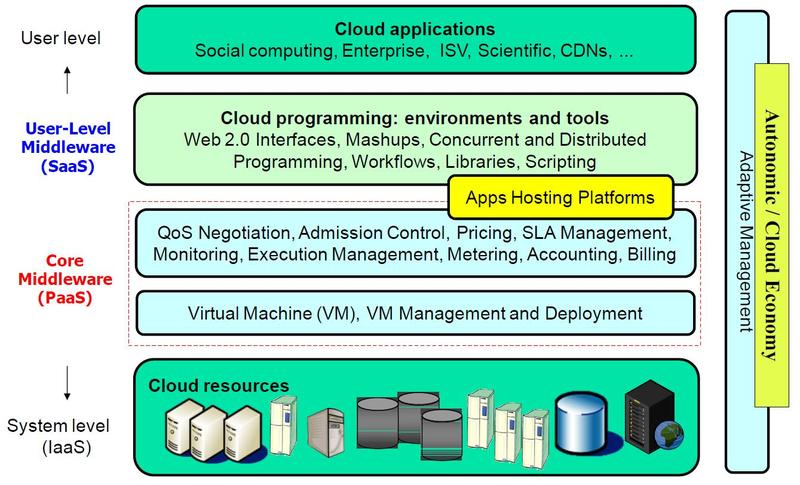
\includegraphics[width=0.7\textwidth]{../plots/cloud_architecture}
    \label{cloud_arch}
  \end{figure*}
  
  The global architecture of a cloud is described in the
  \figurename~\ref{cloud_arch}. It is split in different layers and each layer
  has a specific role in the business model of clouds. On the lowest part there
  is the physical resources (e.g. data centers) with Infrastructure as a Service
  model (IaaS). The pricing is based of the resources available. Then comes the
  layer of virtualization and performances negotiation called Platform as a
  Service (PaaS). Dealing with Virtual Machines (VMs also called hosts) allows a
  cleaner sharing of resources and makes it easier answering the users' demands
  (e.g. deploying more VMs). The pricing depends of multiple factors, like the
  Quality of Service (QoS) for the quality of the network, the Service Level
  Agreement (SLA) for the faults rate, handling and responsibilities... On top
  of that is the layer for users' cloud tools with Software as a Service (SaaS).
  These tools will allow the user that writes cloud applications to manage
  resources, run their code...
  
  Most cloud applications will have fluctuating workload over time. For example 
  with a website server the usage might be bigger during the day or during a 
  short period because of a viral cultural event. Resources should thus be 
  managed dynamically. Also, physical resources can encounter problems which 
  makes them unavailable. Because of all these constraints the SLAs and QoS 
  negotiations aren't satisfied easily and 100\% availability is never a thing. 
  On top of that every actor wants to meet the obligations with a minimal cost. 
  All these questions of availability and cost are current research problems. 
  In particular we are interested in the works that tackle problems related to 
  fluctuating and dynamic usage of cloud applications and resources. The 
  ability for a cloud infrastructure to adapt to a dynamic workload is called 
  cloud elasticity.
  
  There are some generic elastic actions. The act of deploying more VMs (and
  thus having more resources overall) is called scaling up (and the convert is
  scaling down). The act of moving VMs to a different location is called scaling
  out. This is used for example when time passes by and users come from
  different countries/continents.
  
  \cite{Naskos2016} has categorized works on cloud elasticity and allows to see
  which elements of a cloud infrastructure, platform or application/software are
  impacted. As it is for now most research works are evaluated on real clouds.
  It is interesting for a distributed systems simulator to search what is needed
  for simulating cloud elasticity. If it is shown that research works on cloud
  elasticity can be evaluated on a simulator they would benefit from cost
  reduction, re-runable experiments, trust in results...
  
  In this survey proposals are categorized as follows. The scope is about what
  elements of a cloud the proposals work on. It can be the management of VMs,
  allocation of resources... Then there is the purpose of the proposal.
  Enhancing the \textit{performances} (to meet the SLA), reducing the
  \textit{energy consumption} footprint, being \textit{available} when needed
  and reducing the overall \textit{cost}. Another dimension is the decision
  making. This is what a proposal add to an existing cloud to reach its goal. In
  addition to the scope there is the elastic actions performed by the proposals.
  As the scope is about what elements of a cloud are concerned, the elastic
  action is about what is done to them. Then there is the provider dimension
  that tells if there is only one provider or multiple ones. At last there is
  the method used by the proposal to evaluate itself, through real cloud,
  simulation or emulation.
  
  The survey gives a good overview on what elements of a cloud are manipulated
  to achieve cloud elasticity. No clue have been found proving the opposite at
  the time of writing.
  
  As the proposals are on reacting to variating usage, simulators need a way to
  express this fluctuating workload. We worked on elastic tasks that model tasks
  that are triggered regularly and with a usage that fluctuates over time.


\section{State of the art} \label{sota}
  Based on the classification of the survey, a simulator should allow the
  manipulation of scopes, the evaluation of the different purposes, make
  possible the elastic actions and allow multiple providers.
  
  At the moment no simulator article talks about dynamic workload. On the other
  hand in the code of DCsim \cite{tighe2013towards} there was an interactive
  task and in the code of CloudSim \cite{calheiros2011cloudsim} there was an
  host with dynamic workload. There are some tools to generate artificial
  workload like \cite{bodik2010characterizing} and they generally follow the
  following steps. They have a thread that acts like clients/users and it makes
  request over time and simulate times of thinking of the users.
  
  On a less technical note, workloads are generally seen as a number of 
  requests per a certain interval of time.
  
  Five papers in the survey used simulations. They used discrete event 
  simulators (home-made or OMNeT++), used benchmarks like SPECjEnterprise2010 
  to have close-to-reality hosts, and run real traces.
  
%  \begin{center}
%  	\begin{tabular}{| l | c | c | c | c |}
%  		\hline
%  		Paper & Horizontal scaling & Vertical scaling & blabla & blabla \\ 
%  		\hline
%  		\cite{vasic2012dejavu} & \checkmark & \checkmark & & \\
%  		\hline
%  	\end{tabular}
%  \end{center}


\section{Contribution} \label{contrib}
  The work was done on SimGrid \cite{casanova:hal-01017319}. The code is
  available here: \url{https://github.com/sbihel/internship_simgrid}. It was
  written as a plug-in on top of the S4U interface which is intended to be the
  core API. Elastic tasks are objects and are the only things the user has to
  manipulate.
  
  An elastic task can repeat a certain task that we will call microtask. The 
  user provides a rate of triggering per second and the flops required and then 
  over time multiple identical microtasks will be created and executed. An 
  elastic task can have multiple hosts to split the workload and there will be 
  a cycling shifting between hosts when creating microtasks, keeping one host 
  for one microtask.
  
  An output function can be provided to an elastic task and this function will 
  be executed after each microtask that has ended. This has multiple usages. It 
  allows the description of workflows of tasks. As microtasks only generate 
  computing workload, output functions can be used to have different types of 
  workloads like network usage, disk access (which can be simulated only by 
  seeing it as a particular computing resource at the moment), and basically 
  anything possible with SimGrid.
  
  It is also useful to study the behavior of a system dealing with real 
  workload. For that an elastic task can be given a file of timestamps and it 
  will trigger/generate a microtask for each time stamp.
  
  For detailed platforms description it is a core feature of SimGrid which 
  allows to have multiple providers, topologies, hosts (VMs for us), 
  bandwidths...


\section{Evaluation} \label{eval}
  The contribution has been evaluated on the predefined criteria. We first did 
  an experiment for raw performances. Then we used real traces from WorldCup 98 
  data access logs \cite{wc98} which are often used. After that we evaluated 
  the expressiveness and functionalities. All experiments have been executed on 
  a MacBook Pro with an Intel Core i5 and 8GB of RAM.
    
  \subsection{Raw performances} \label{raw_perf}
    \begin{figure}
      \caption{Raw performances CPU time}
      \centering
      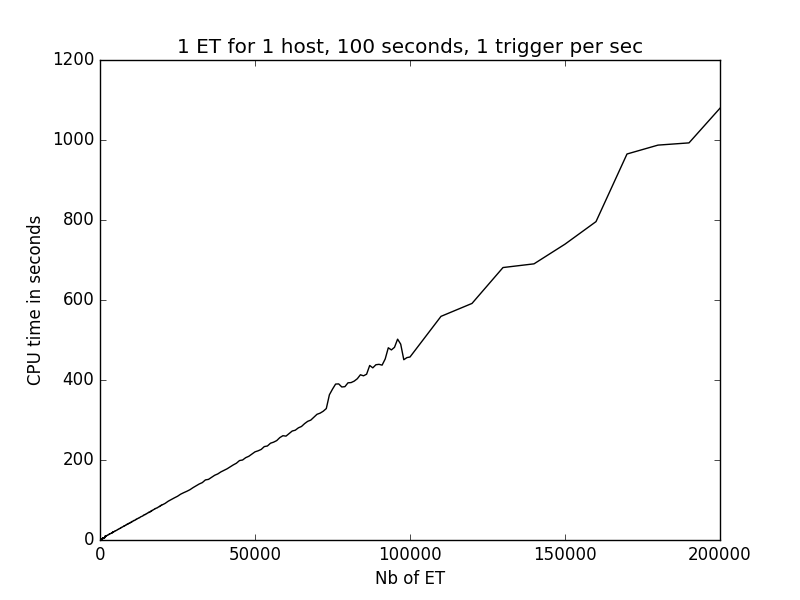
\includegraphics[width=0.55\textwidth]{../plots/raw_perf_time}
      \label{time_raw}
    \end{figure}
    \begin{figure}
      \caption{Raw performances Max Memory}
      \centering
      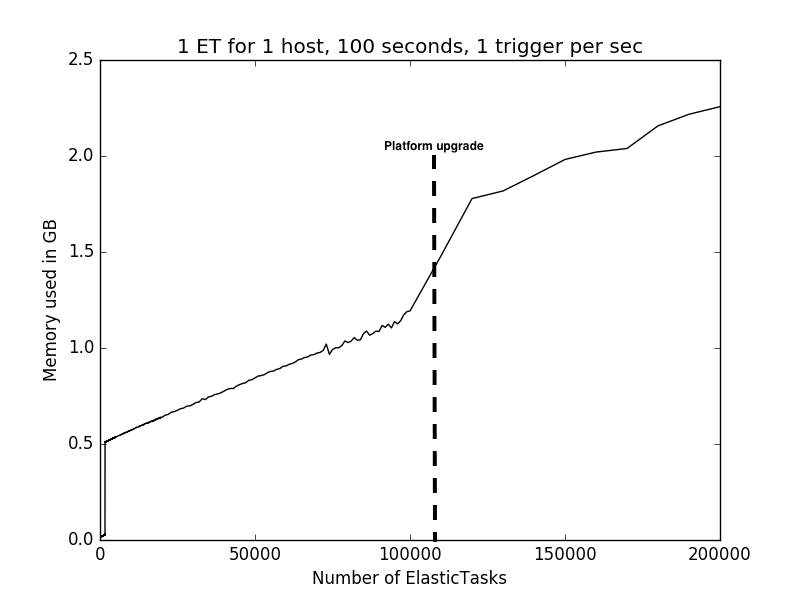
\includegraphics[width=0.55\textwidth]{../plots/raw_perf_mem}
      \label{mem_raw}
    \end{figure}
    
    \figurename~\ref{time_raw} shows the CPU time (user + system time) while 
    \figurename~\ref{mem_raw} shows the maximum memory used. The platform was
    upgraded two times, at 1,600 from 2,000 hosts to 100,000, and then at
    100,000 from 100,000 to 200,000. We can see that the deployment of the 
    platform has nearly no impact on the time but account for about a half of 
    the memory used if there is as much ETs as hosts. Apart from that time and 
    memory grows linearly depending of the ETs amounts and operations done.
    
    % for the spikes in CPU it might be because I was doing other stuff with my 
    % laptop
    % exceeding computing capacities of hosts might slow things
    
  \subsection{Real traces}
    For that we used real traces from WorldCup 98 data access logs \cite{wc98}
    with a platform of 2,000 host and enough flops. After translating the
    requests log as a timestamps file we tested with the test file of 1,000. It
    took 0.14 seconds of CPU time and 13,484 KB. Then with the same platform we
    used the days 10 and 20 with respectively 1,522,111 and 6,326,015 requests.
    The first one took 50.82 seconds of CPU time and 13,876 KB of memory and
    the later took 229.62 seconds and 14,472 KB. Adding more hosts changed 
    except for the deployment of the platform as we have seen in \ref{raw_perf}.
  
  \subsection{Functionalities}
   For horizontal and vertical scalings, they can be performed by modifying the 
   list of hosts of an ET. To scale up you just have to add hosts and to scale 
   out you have to replace this list with different hosts. Concerning workflows 
   of tasks you can set the output function with a function that has access to 
   ETs you want to trigger and just trigger them in the function, with possibly 
   a multiplicative effect of the workload.
  

% \section{Future work} \label{futurework}
% generator law, add natively other kinds of workload instead of letting the 
% user do some kinds of hacks
  

\section{Conclusion} \label{conclu}
During this internship we've studied which actions were taken by elastic clouds 
mechanisms. Then we searched what was done in simulations used for evaluations 
and other evaluations to come with a contribution that meets the needs of 
researchers. To prove that the contribution was good enough we evaluated it on 
some criteria.

% tho there is still work to do ?


\bibliographystyle{IEEEtran}
\bibliography{bibi}
\end{document}
